\documentclass[a4paper,12pt,twoside]{memoir}

% Castellano
\usepackage[spanish,es-tabla]{babel}
\selectlanguage{spanish}
\usepackage[utf8]{inputenc}
\usepackage[T1]{fontenc}
\usepackage{lmodern} % Scalable font
\usepackage{microtype}
\usepackage{placeins}

\RequirePackage{booktabs}
\RequirePackage[table]{xcolor}
\RequirePackage{xtab}
\RequirePackage{multirow}

% Links
\usepackage[colorlinks]{hyperref}
\hypersetup{
	allcolors = {blue}
}

% Ecuaciones
\usepackage{amsmath}

% Rutas de fichero / paquete
\newcommand{\ruta}[1]{{\sffamily #1}}

% Párrafos
\nonzeroparskip


% Imagenes
\usepackage{graphicx}
\newcommand{\imagen}[2]{
	\begin{figure}[!h]
		\centering
		\includegraphics[width=0.9\textwidth]{#1}
		\caption{#2}\label{fig:#1}
	\end{figure}
	\FloatBarrier
}

\newcommand{\imagenflotante}[2]{
	\begin{figure}%[!h]
		\centering
		\includegraphics[width=0.9\textwidth]{#1}
		\caption{#2}\label{fig:#1}
	\end{figure}
}



% El comando \figura nos permite insertar figuras comodamente, y utilizando
% siempre el mismo formato. Los parametros son:
% 1 -> Porcentaje del ancho de página que ocupará la figura (de 0 a 1)
% 2 --> Fichero de la imagen
% 3 --> Texto a pie de imagen
% 4 --> Etiqueta (label) para referencias
% 5 --> Opciones que queramos pasarle al \includegraphics
% 6 --> Opciones de posicionamiento a pasarle a \begin{figure}
\newcommand{\figuraConPosicion}[6]{%
  \setlength{\anchoFloat}{#1\textwidth}%
  \addtolength{\anchoFloat}{-4\fboxsep}%
  \setlength{\anchoFigura}{\anchoFloat}%
  \begin{figure}[#6]
    \begin{center}%
      \Ovalbox{%
        \begin{minipage}{\anchoFloat}%
          \begin{center}%
            \includegraphics[width=\anchoFigura,#5]{#2}%
            \caption{#3}%
            \label{#4}%
          \end{center}%
        \end{minipage}
      }%
    \end{center}%
  \end{figure}%
}

%
% Comando para incluir imágenes en formato apaisado (sin marco).
\newcommand{\figuraApaisadaSinMarco}[5]{%
  \begin{figure}%
    \begin{center}%
    \includegraphics[angle=90,height=#1\textheight,#5]{#2}%
    \caption{#3}%
    \label{#4}%
    \end{center}%
  \end{figure}%
}
% Para las tablas
\newcommand{\otoprule}{\midrule [\heavyrulewidth]}
%
% Nuevo comando para tablas pequeñas (menos de una página).
\newcommand{\tablaSmall}[5]{%
 \begin{table}
  \begin{center}
   \rowcolors {2}{gray!35}{}
   \begin{tabular}{#2}
    \toprule
    #4
    \otoprule
    #5
    \bottomrule
   \end{tabular}
   \caption{#1}
   \label{tabla:#3}
  \end{center}
 \end{table}
}

%
% Nuevo comando para tablas pequeñas (menos de una página).
\newcommand{\tablaSmallSinColores}[5]{%
 \begin{table}[H]
  \begin{center}
   \begin{tabular}{#2}
    \toprule
    #4
    \otoprule
    #5
    \bottomrule
   \end{tabular}
   \caption{#1}
   \label{tabla:#3}
  \end{center}
 \end{table}
}

\newcommand{\tablaApaisadaSmall}[5]{%
\begin{landscape}
  \begin{table}
   \begin{center}
    \rowcolors {2}{gray!35}{}
    \begin{tabular}{#2}
     \toprule
     #4
     \otoprule
     #5
     \bottomrule
    \end{tabular}
    \caption{#1}
    \label{tabla:#3}
   \end{center}
  \end{table}
\end{landscape}
}

%
% Nuevo comando para tablas grandes con cabecera y filas alternas coloreadas en gris.
\newcommand{\tabla}[6]{%
  \begin{center}
    \tablefirsthead{
      \toprule
      #5
      \otoprule
    }
    \tablehead{
      \multicolumn{#3}{l}{\small\sl continúa desde la página anterior}\\
      \toprule
      #5
      \otoprule
    }
    \tabletail{
      \hline
      \multicolumn{#3}{r}{\small\sl continúa en la página siguiente}\\
    }
    \tablelasttail{
      \hline
    }
    \bottomcaption{#1}
    \rowcolors {2}{gray!35}{}
    \begin{xtabular}{#2}
      #6
      \bottomrule
    \end{xtabular}
    \label{tabla:#4}
  \end{center}
}

%
% Nuevo comando para tablas grandes con cabecera.
\newcommand{\tablaSinColores}[6]{%
  \begin{center}
    \tablefirsthead{
      \toprule
      #5
      \otoprule
    }
    \tablehead{
      \multicolumn{#3}{l}{\small\sl continúa desde la página anterior}\\
      \toprule
      #5
      \otoprule
    }
    \tabletail{
      \hline
      \multicolumn{#3}{r}{\small\sl continúa en la página siguiente}\\
    }
    \tablelasttail{
      \hline
    }
    \bottomcaption{#1}
    \begin{xtabular}{#2}
      #6
      \bottomrule
    \end{xtabular}
    \label{tabla:#4}
  \end{center}
}

%
% Nuevo comando para tablas grandes sin cabecera.
\newcommand{\tablaSinCabecera}[5]{%
  \begin{center}
    \tablefirsthead{
      \toprule
    }
    \tablehead{
      \multicolumn{#3}{l}{\small\sl continúa desde la página anterior}\\
      \hline
    }
    \tabletail{
      \hline
      \multicolumn{#3}{r}{\small\sl continúa en la página siguiente}\\
    }
    \tablelasttail{
      \hline
    }
    \bottomcaption{#1}
  \begin{xtabular}{#2}
    #5
   \bottomrule
  \end{xtabular}
  \label{tabla:#4}
  \end{center}
}



\definecolor{cgoLight}{HTML}{EEEEEE}
\definecolor{cgoExtralight}{HTML}{FFFFFF}

%
% Nuevo comando para tablas grandes sin cabecera.
\newcommand{\tablaSinCabeceraConBandas}[5]{%
  \begin{center}
    \tablefirsthead{
      \toprule
    }
    \tablehead{
      \multicolumn{#3}{l}{\small\sl continúa desde la página anterior}\\
      \hline
    }
    \tabletail{
      \hline
      \multicolumn{#3}{r}{\small\sl continúa en la página siguiente}\\
    }
    \tablelasttail{
      \hline
    }
    \bottomcaption{#1}
    \rowcolors[]{1}{cgoExtralight}{cgoLight}

  \begin{xtabular}{#2}
    #5
   \bottomrule
  \end{xtabular}
  \label{tabla:#4}
  \end{center}
}


















\graphicspath{ {./img/} }

% Capítulos
\chapterstyle{bianchi}
\newcommand{\capitulo}[2]{
	\setcounter{chapter}{#1}
	\setcounter{section}{0}
	\chapter*{#2}
	\addcontentsline{toc}{chapter}{#2}
	\markboth{#2}{#2}
}

% Apéndices
\renewcommand{\appendixname}{Apéndice}
\renewcommand*\cftappendixname{\appendixname}

\newcommand{\apendice}[1]{
	%\renewcommand{\thechapter}{A}
	\chapter{#1}
}

\renewcommand*\cftappendixname{\appendixname\ }

% Formato de portada
\makeatletter
\usepackage{xcolor}
\newcommand{\tutor}[1]{\def\@tutor{#1}}
\newcommand{\course}[1]{\def\@course{#1}}
\definecolor{cpardoBox}{HTML}{E6E6FF}
\def\maketitle{
  \null
  \thispagestyle{empty}
  % Cabecera ----------------
\noindent
\includegraphics[width=\textwidth]{cabecera}\vspace{1cm}%
  \vfill
  % Título proyecto y escudo informática ----------------
  \colorbox{cpardoBox}{%
    \begin{minipage}{.8\textwidth}
      \vspace{.5cm}\Large
      \begin{center}
      \textbf{TFG del Grado en Ingeniería Informática}\vspace{.6cm}\\
      \textbf{\LARGE\@title{}}
      \end{center}
      \vspace{.2cm}
    \end{minipage}

  }%
  \hfill\begin{minipage}{.20\textwidth}
    
\includegraphics[width=\textwidth]{escudoInfor}
  \end{minipage}
  \vfill
  % Datos de alumno, curso y tutores ------------------
  \begin{center}%
  {%
    \noindent\LARGE
    Presentado por \@author{}\\ 
    en Universidad de Burgos --- \@date{}\\
    Tutor: \@tutor{}\\
  }%
  \end{center}%
  \null
  \cleardoublepage
  }
\makeatother

\newcommand{\nombre}{Mario de la Parte Izquierdo} %%% cambio de comando

% Datos de portada
\title{Sistema de Información sobre Matriculación}
\author{\nombre}
\tutor{Carlos Pardo Aguilar}
\date{\today}

\begin{document}

\maketitle


\newpage\null\thispagestyle{empty}\newpage


%%%%%%%%%%%%%%%%%%%%%%%%%%%%%%%%%%%%%%%%%%%%%%%%%%%%%%%%%%%%%%%%%%%%%%%%%%%%%%%%%%%%%%%%
\thispagestyle{empty}


\noindent
\includegraphics[width=\textwidth]{cabecera}\vspace{1cm}

\noindent D. Carlos Pardo Aguilar, profesor del departamento de Ingeniería Civil, área de Lenguajes y Sistemas Informáticos.

\noindent Expone:

\noindent Que el alumno D. \nombre, con DNI 71305494C, ha realizado el Trabajo final de Grado en Ingeniería Informática titulado \emph{Sistema de Información sobre Matriculación}. 

\noindent Y que dicho trabajo ha sido realizado por el alumno bajo la dirección del que suscribe, en virtud de lo cual se autoriza su presentación y defensa.

\begin{center} %\large
En Burgos, {\large \today}
\end{center}

\vfill\vfill\vfill

% Author and supervisor
%\begin{minipage}{0.45\textwidth}
%\begin{flushleft} %\large
%Vº. Bº. del Tutor:\\[2cm]
%D. Carlos Pardo Aguilar
%\end{flushleft}
%\end{minipage}
%\hfill

%\begin{minipage}{0.45\textwidth}
%\begin{flushleft} %\large
%Vº. Bº. del co-tutor:\\[2cm]
%D. nombre co-tutor
%\end{flushleft}
%\end{minipage}
%\hfill


% para casos con solo un tutor comentar lo anterior
% y descomentar lo siguiente
\begin{minipage}{0.45\textwidth}
\begin{flushleft} %\large
Vº. Bº. del Tutor:\\[2cm]
D. Carlos Pardo Aguilar
\end{flushleft}
\end{minipage}
\hfill


\vfill

\newpage\null\thispagestyle{empty}\newpage




\frontmatter

% Abstract en castellano
\renewcommand*\abstractname{Resumen}
\begin{abstract}
En este primer apartado se hace una \textbf{breve} presentación del tema que se aborda en el proyecto.
\end{abstract}

\renewcommand*\abstractname{Descriptores}
\begin{abstract}
Preprocesado Sigma, Sistema de Información, Matrícula
\end{abstract}

\clearpage

% Abstract en inglés
\renewcommand*\abstractname{Abstract}
\begin{abstract}
A \textbf{brief} presentation of the topic addressed in the project.
\end{abstract}

\renewcommand*\abstractname{Keywords}
\begin{abstract}
Preprocessed Sigma, Information System, Enrollment
\end{abstract}

\clearpage

% Indices
\tableofcontents

\clearpage

\listoffigures

\clearpage

\listoftables
\clearpage

\mainmatter
\capitulo{1}{Introducción}

%Descripción del contenido del trabajo y del estrucutra de la memoria y del resto de materiales entregados.

En la actualidad, existe una gran cantidad de información o datos, los cuales componen una parte muy importante en las grandes  empresas y organizaciones de todo el mundo.
Cada día se genera multitud de nueva información y es indispensable almacenarla para posteriormente poder interpretarla correctamente. Es imprescindible por lo tanto, saber extraer e identificar información relevante a partir de ficheros o documentos poco legibles o difíciles de entender a priori.


En este punto es cuando toma especial interés la creación de un Sistema de Información, o lo que es lo mismo, un almacén electrónico. En dichos almacenes se protege y mantiene una gran cantidad de datos e información, de manera fiable, segura y fácil de administrar.

Además de estas funciones de almacenamiento y administración, un Sistema de Información también permite organizar, entender y utilizar los datos para la toma de decisiones.
Para esta tarea, es necesario contar con cierta capacidad de análisis, ya que hay que extraer información concreta, destacada y relevante; para posteriormente poder visualizarla con ayuda de elementos visuales como gráficos.

En la realización de este proyecto se propone la creación de un Sistema de Información, para procesar, almacenar y representar visualmente la información sobre la matriculación de alumnos en la Universidad de Burgos. 


De esta forma, en el proyecto se podrán diferenciar varias funcionalidades:

\begin{itemize}
	\item Preprocesamiento de los ficheros Excel(.xls) descargados de Sigma.
	\item Creación de la Base de Datos(BBDD).
	\item Carga de datos en la Base da Datos(BBDD) a partir de los ficheros(.csv) generados.
	\item Visualización de diferentes tipos de gráficos en función de los datos de la BBDD y lo que el usuario seleccione.
\end{itemize}


\section{Estructura de la memoria}\label{estructura-de-la-memoria}
La memoria se estructura de la siguiente manera:

\begin{itemize}
\item 
\textbf{Introducción:} se describe brevemente el contexo y el proyecto realizado. Posteriormente se realiza una sección donde se expone la estructura de la memoria.

\item 
\textbf{Objetivos del proyecto:} se exponen los objetivos del proyecto, divididos en objetivo general y objetivos técnicos.


%\item
%\textbf{Conceptos teóricos:} se exponen los conceptos básicos para comprender tanto el proyecto como el desarrollo del mismo.
\item
\textbf{Técnicas y herramientas:} se explican las metodologías y herramientas utilizadas durante el desarrollo del proyecto.
%\item
%\textbf{Trabajos relacionados:} se exponen aplicaciones, proyectos y empresas que ofrecen soluciones en un campo similar al caso de estudio.
%\item
%\textbf{Conclusiones y líneas de trabajo futuras:} se explican las conclusiones finales que se obtienen después de la realización del proyecto, así como futuras mejoras.
\end{itemize}
\capitulo{2}{Objetivos del proyecto}

A continuación se definen los objetivos del proyecto realizado, divididos en tres apartados:


\section{Objetivo general}\label{objetivo-general}

\begin{itemize}

\item
  Desarrollar una aplicación para analizar datos relacionados con la matriculación de alumnos en la Universidad de Burgos (UBU).
  
\end{itemize}



\section{Objetivos técnicos}\label{objetivos-tecnicos}

\begin{itemize}

\item
  Extraer los datos o información relevante de ficheros Excel (.xls), utilizando librerías concretas de Python.
\item
  Crear las diferentes bases de datos para almacenar los datos anteriormente extraídos. 
\item
  Identificar y crear gráficos o estadísticos que resulten útiles para visualizar y comparar información.
\item
  Desarrollar una aplicación en Python que unifique todo lo anterior, así como realizar una la interfaz gráfica agradable para el usuario.

\end{itemize} 

  
\section{Objetivos personales}\label{objetivos-personales}

\begin{itemize}

\item
  Adquirir conocimiento sobre la extracción de grandes cantidades de datos de ficheros y creación de bases de datos.
\item
  Profundizar en el conocimiento sobre análisis de datos y gestión de la información.


\end{itemize}


%\capitulo{3}{Conceptos teóricos}

En este apartado se van a explicar aquellos conceptos teóricos básicos que son necesarios para comprender el proyecto.


\section{Sistema de Información}



\subsection{Definición}

Para comenzar, hay que explicar que no existe una definición de consenso en la propia definición de Sistema de Información. De hecho, existen multitud de definiciones diferentes sobre cómo se define un Sistema de Información.


Los autores Laudon y Laudon definen un Sistema de Información como un conjunto de módulos relacionados ente sí que son capaces de obtener(o reutilizar), procesar, almacenar y distribuir cierta información para que sirva de apoyo para la toma de decisiones \cite{vicen}.
A parte de suministrar apoyo en decisiones importantes, también pueden ayudar a detectar problemas o carencias difíciles de ver sin la ayuda de estos sistemas.


\subsection{Componentes de un Sistema de Información}
Aunque existen numerosas definiciones y no existe una definición general o global, la mayoría de Sistemas de Información pueden representarse a través del siguiente diagrama:

\imagen{componentesSI}{Componentes de un Sistema de Información}
Se pueden apreciar 5 elementos principales. En primer lugar los elementos de entrada, que en nuestro proyecto serían los ficheros (.xls) originales descargados de \emph{Sigma}. 

A continuación estaría un elemento de modificación o transformación, que en nuestro caso sería el preprocesado de los ficheros originales anteriores en ficheros (.csv) reordenados, modificados y sin ningún tipo de error. También se podría incluir la carga de datos a la Base de Datos creada con anterioridad.

Seguidamente estaría el sistema de salida, donde se visualizan los resultados obtenidos. En este proyecto, el sistema de salida serían los diferentes tipos de gráficos que se pueden obtener a partir de la información que seleccione el usuario y los datos existentes o disponibles en la BBDD.

Además de estas 3 secciones, se aprecian otras dos secciones más. Una de ellas es el mecanismo de control, que es el proceso encargado de lograr los objetivos, que sería el quinto y último elemento.
En nuestro proyecto se podrían identificar numerosos mecanismos de control, como por ejemplo que los ficheros que se puedan seleccionar en los botones de \emph{Preprocesar} y \emph{Cargar Archivos} sean únicamente (.xls) y (.csv) respectivamente. Otros mecanismos de control serían la no introdución de datos repetidos en la BBDD o la selección de opciones de datos que realmente se encuentran en la BBDD, entre otros.

En cuanto a los objetivos de nuestro sistema de información, hay que destacar que se definen en el apartado anterior denominado \emph{Objetivos del proyecto}.

\subsection{Características de un Sistema de Información}



\subsection{Tipos de Sistemas de Información}



\subsection{Ventajas de un Sistema de Información}



\section{Parseado de Datos}
El Preprocesado / Parseado de ficheros es un proceso mediante el cual...




\section{Base de datos}
Una base de datos es ...

\section{Aplicación de escritorio}

\section{Gráficos Representados}


\subsection{Gráfico de Barras}

\subsection{Gráfico de Cuartiles}

\begin{itemize}
	\item Max.
	\item Min.
	\item Media.
\end{itemize}


%\capitulo{4}{Técnicas y herramientas}

En este apartado se van a exponer las técnicas metodológicas y herramientas de desarrollo que se han utilizado para la realización del proyecto. Se detallarán las razones principales por los que se ha usado esa herramienta y no otra.

\section{Metodologías}\label{metodologias}

\subsection{Scrum}\label{scrum}
Para realizar la planificación correcta del proyecto, se ha utilizado \emph{Scrum}, que es una metodología ágil de desarrollo.

\begin{itemize}
	\item Se ha utilizado una estrategia orientada a un desarrollo incremental y basada en \emph{sprints}.
	\item La duración media de cada \emph{sprint} era aproximadamente de una semana.
	\item Al inicio de cada \emph{sprint} se definían las tareas o \emph{issues} a realizar, las cuales tenían que ser realizadas en un cierto intervalo de tiempo.
	\item Cada \emph{sprint} se planificaba cuando se finalizaban las tareas o \emph{issues} del anterior \emph{sprint}.	
	\item Al final de cada \emph{sprint} se revisan todas las tareas realizadas, así como ver si se han logrado los objetivos fijados y solucionado los problemas encontrados.
\end{itemize}

Con la utilización de esta metodología se ha logrado evitar la realización de una planificación y ejecución completa desde el inicio del proyecto.


\section{Lenguaje de Programación}\label{lenguaje_de_programacion}
\subsection{Python}\label{python}
El lenguaje de programación utilizado ha sido Python\footnote{\href {http://www.python.org/}{www.python.org}} en la versión 3.7.1.

Las razones por las que se ha decidido utilizar Python son las siguientes:
\begin{itemize}
	\item Es uno de los lenguajes de programación más sencillos de aprender ya que su sintaxis es muy entendible.
	\item Es un lenguaje gratuito, multiplataforma y de código abierto.
	\item Gracias a las dos anteriores razones, se ha convertido en un lenguaje tan popular y utilizado, que ha dado lugar a que se desarrollen multitud de librerías, módulos y programas de software libre. Gran parte de estas librerías destacan en el ámbito de manejo de ficheros, tratamiento y visualización de datos.
	\item Del mismo modo, al ser un lenguaje utilizado por tantas personas, hace que existan numerosos foros, blogs y páginas en las que apoyarse cuando surgen dudas o se necesita ayuda.
\end{itemize}


\section{Entorno de Desarrollo}\label{entorno_de_desarrollo}
\subsection{Jupyter NoteBook}\label{jupyter_noteBook}
Como entorno de desarrollo principal se ha utilizado Juypter NoteBook\footnote{\href {https://jupyter.org/}{www.jupyter.org}} en la versión 5.7.4.

Se trata de una aplicación web de código abierto que permite tanto el desarrollo como la ejecución del código.
Esta aplicación se puede lanzar directamente desde un navegador(sin instalar nada) o se puede instalar con \emph{Anaconda Navigator}. Para el desarrollo del proyecto se utilizó la segunda opción.

Otra de las grandes ventajas de esta aplicación es la agilidad en el desarrollo, ya que al tratarse de una aplicación cuya ejecución es en vivo, se pueden realizar pruebas de manera rápida e intuitiva. 


\subsection{SQLite}\label{sqlite}
SQLite\footnote{\href {https://www.sqlite.org/index.html}{www.sqlite.org}} se trata de un sistema de gestión de bases de datos(BBDD) relacionales de pequeño tamaño.
Una de las características de este sistema de gestión es que no necesita un servidor para poder utilizarse, ya que los datos se almacenan en un único fichero en el sistema host. 
Hay que destacar que Python incluye soporte para SQLite desde la versión 2.5 incorporado en la Biblioteca Estándar como el módulo \emph{sqlite3}, que es el módulo que se ha utilizado en el desarrollo del proyecto \cite{sqlite}.



\section{Control de Versiones}\label{control_de_versiones}
\subsection{GitHub}\label{gitHub}
GitHub\footnote{\href {https://github.com/}{www.github.com}} se trata de una plataforma cuya función principal es la de hospedar repositorios y permitir el desarrollo colaborativo.
Es una plataforma de las más usadas y por esta razón es la que se ha utilizado a lo largo del grado y en particular en la realización de este proyecto. Hay que destacar que gracias a formar parte de la Universidad de Burgos y ser estudiante, se ha obtenido la versión \emph{PRO}(licencia de estudiantes). Aun así hay que destacar que se trata de una herramienta gratuita.
Por último comentar que se ha utilizado tanto \emph{GitHub Desktop}(aplicación de escritorio) como la plataforma web.



\section{Documentación}\label{documentacion}

\subsection{Texmaker}\label{texmaker}
Para la realización de la documentación con \LaTeX\footnote{\href {https://www.latex-project.org/}{www.latex-project.org}} se ha utilizado el editor Texmaker\footnote{\href {https://www.xm1math.net/texmaker/}{www.xm1math.net/texmaker}}. Se trata de un editor gratuito, el cual contiene las herramientas y características necesarias para desarrollar y editar documentos con \LaTeX.

Hay que señalar que también incluye corrección ortográfica, auto-completado, plegado de código y un visor incorporado en pdf con soporte de synctex y un modo de visualización continua \cite{texmaker}. 



\section{Otras Herramientas}\label{otras_herramientas}
En este apartado se van a explicar otras herramientas destacadas que se han utilizado a lo largo del proyecto.

\subsection{DB Browser}\label{db_browser}
DB Browser\footnote{\href{https://sqlitebrowser.org/}{www.sqlitebrowser.org}} es una herramienta gratuita y de código abierto cuyo principal objetivo es la administración de Bases de Datos que utilizan SQLite como motor de las mismas. Esta herramienta cuenta con numerosas funcionalidades, entre las que se encuentran la creación de BBDD, tablas, índices, entradas, importar y exportar archivos, entre otras.

Hay que destacar que en este proyecto se ha utilizado la aplicación de escritorio para tareas de visualización de datos de la BBDD y comprobación de los mismos.


\subsection{Sublime Text 3 y Notepad++}\label{sublime_text_3_y_notepad++}
Tanto Sublime Text 3\footnote{\href{https://www.sublimetext.com/}{www.sublimetext.com}} como Notepad++\footnote{\href{https://notepad-plus-plus.org/}{www.notepad-plus-plus.org}} son editores de código que pueden ser utilizados como entornos de desarrollo, ya que pueden interpretar numerosos lenguajes de programación. 

En un primer lugar ambos editores se utilizaron para el desarrollo del proyecto, pero finalmente el uso de estas herramientas fue la de edición y visualización de ficheros. Hay que destacar funcionalidades como la mostrar caracteres ocultos de \emph{Notepad++}, la visualización del texto en función de la sintaxis o lenguaje de programación que se elija en \emph{Sublime Text 3} y las herramientas de búsqueda de ambos editores.

\subsection{Nitro Pro}\label{nitro_pro}
Nitro Pro\footnote{\href{https://www.gonitro.com/es/}{www.gonitro.com}} es una herramienta gráfica cuya funcionalidad reside en la creación y edición de ficheros (.pdf). Hay que destacar que al tratarse de una herramienta de pago, se ha utilizado la versión de prueba de la misma, ya que contaba con las funcionalidades necesarias para el proyecto.

Esta herramienta se ha utilizado para la edición de ficheros (.pdf) como \emph{about.pdf} de la interfaz gráfica.

\subsection{Excel}\label{excel}
Excel\footnote{\href{https://support.office.com/es-es/excel}{www.support.office.com/es-es/excel}} pertenece a la categoría de programas conocidos como hojas de cálculo \cite{excel}.

De hecho es una de las herramientas más utilizadas y potentes en el análisis de datos, ya que cuenta con una gran cantidad de funcionalidades relacionadas con este área.

En la realización del proyecto, se ha utilizado principalmente para modificar(pruebas) y visualizar tanto los ficheros originales (.xls), como los generados (.csv). 


\subsection{Photoshop}\label{photoshop}
Photoshop\footnote{\href{https://www.photoshop.com/}{www.photoshop.com}} es un editor de imágenes dedicado principalmente para el retoque de fotografías y creación de gráficos. 

Esta herramienta se ha utilizado para pequeñas tareas de diseño gráfico, como la realización de los botones de tipos de gráfico, el logotipo de la aplicación...etc.
\capitulo{5}{Aspectos relevantes del desarrollo del proyecto}

En este apartado se van a recoger los aspectos más importantes que han surgido en el desarrollo del proyecto. Se incluirán la toma de decisiones, los posibles cambios, la aparición de problemas y las soluciones establecidas.

\section{Inicio del proyecto}\label{inicio_del_proyecto}

Al principio se propuso la idea de la creación de una variante de \emph{Data Ware-House} o almacén de datos, para almacenar información relevante para la matriculación de alumnos en la Universidad de Burgos(UBU) y su futura utilización para la toma de decisiones.

La idea transmitida por el tutor fue la creación de un sistema para poder almacenar y visualizar cualquier grado o máster de la UBU.

El tutor comentó que los archivos que se iban a utilizar de partida, eran un tipo de ficheros descargado desde una aplicación denominada \emph{Sigma}.


...





\includegraphics[ scale = 0.60]{errorFicheroOriginal}
%\imagen{errorFicheroOriginal}{Error al intentar abrir con Excel los ficheros originales}


\section{Metodologías}\label{metodologias}

A lo largo del desarrollo del proyecto se ha usado la \emph{metodología Scrum}. Se trata de una metodología ágil basada en \emph{sprints}, en este caso, de desarrollo incremental con revisiones semanales.

Por lo tanto, la duración estimada de cada \emph{sprint} es de una semana, si bien ha habido varios \emph{sprints} que han tenido una duración superior. Al finalizar cada \emph{sprint}, se planificaba el siguiente, creando sus \emph{issues} o tareas a realizar en dicho \emph{sprint}. Cuando estas tareas se realizaban, se cambiaba el estado del \emph{issue} correspondiente a \emph{Closed}.  


\section{Toma de decisiones}\label{toma_de_decisiones}


\section{Librerías para el tratamiento y manipulación de datos}\label{librerias}
En este apartado se van a explicar las diferentes librerías o bibliotecas que se han utilizado en el desarrollo del proyecto y su función principal. Todas las librerías explicadas a continuación son de \emph{Python}.

\subsection{re}
La primera librería que se ha utilizado en el proyecto ha sido re\footnote{\href {https://docs.python.org/3/library/re.html}{www.docs.python.org/3/library/re}}, ya que dicha librería contiene las funciones necesarias para trabajar con expresiones regulares.

Las expresiones regulares se han utilizado sobretodo en la parte inicial de parsear los ficheros descargados de Sigma. De esta manera se ha podido separar y extraer información por filas, celdas y contenido de las mismas.


\subsection{pandas}
Pandas\footnote{\href{https://pandas.pydata.org/}{www.pandas.pydata.org}} es una librería que ofrece numerosas estructuras de datos de gran rendimiento y herramientas de análisis de datos.

Esta librería se ha utilizado principalmente para abrir y crear archivos con \emph{Python} y para crear \emph{dataframes} o estructuras auxiliares donde guardar datos.  


\subsection{sqlite3}
Como ya se ha comentado en un apartado anterior, la librería sqlite3\footnote{\href{https://docs.python.org/2/library/sqlite3.html}{www.docs.python.org/2/library/sqlite3.html}} proporciona una base de datos relacional de pequeño tamaño, ya que no necesita un servidor para poder utilizarse, ya que los datos se almacenan en un único fichero en el sistema host.

Esta librería se ha utilizado para la creación de la base de datos(BBDD), así como para la carga de datos y los procesos de consultas a la misma.

\subsection{Tkinter}
Tkinter\footnote{\href{https://docs.python.org/2/library/tkinter.html}{www.docs.python.org/2/library/tkinter.html}} es una librería con numerosas funciones para hacer posible la creación de una interfaz gráfica en \emph{Python}.

Se trata de una librería orientada a objetos y gracias a su facilidad de uso y rapidez para realizar una GUI, es una de las librerías más destacadas de este lenguaje de programación.

Por lo tanto, se ha utilizado principalmente en la creación de la interfaz gráfica(botones, desplegables, ventanas nuevas...etc).


\subsection{math}
La librería o componente math\footnote{\href{https://docs.python.org/3/library/math.html}{www.docs.python.org/3/library/math.html}} incluye principalmente funciones matemáticas, para realizan operaciones aritméticas. 


\subsection{matplotlib}
La librería matplotlib\footnote{\href{https://matplotlib.org/}{www.matplotlib.org}} cuenta con multitud de funciones y características para generar gráficos. Hay que destacar que se pueden generar una gran variedad de gráficos(de sector, de barras...), así como personalizar los mismos(ejes, etiquetas, fuente, leyenda...)

Esta librería se ha utilizado para la realización y personalización de los gráficos de la interfaz gráfica.


\subsection{os}
La librería os\footnote{\href{https://docs.python.org/3/library/os.html}{www.docs.python.org/3/library/os.html}} de Python permite poder usar funcionalidades relacionadas con el Sistema Operativo. 

Las funciones más destacadas de esta librería y las que se han utilizado son las que informan sobre el entorno del Sistema Operativo y las que permiten navegar por la estructura de directorios, ya sea para leer o modificar archivos.


\section{Interfaz de usuario del proyecto}\label{interfaz_de_usuario_del_proyecto}




\section{Problemas encontrados}

\subsection{Error al abrir los Excel(.xls) bajados de Sigma con Python}
Los archivos Excel(.xls) suministrados (descargados de plataforma \emph{Sigma}) no cumplen el estándar. Al abrirlos tanto con Excel como con varias librerías de Python, muestran un error de formato y extensión. Por lo tanto la única solución encontrada, ha sido realizar un parseo previo de los Excel suministrados, creando un fichero (.csv) nuevo, con toda la información del fichero original corrupto.

De esta manera, se ha creado un analizador sintáctico capaz de leer los ficheros originales (.xls) en modo texto (.xml) y finalmente obtener un (.csv). Se ha parseado toda la información obteniendo filas, celdas, separaciones entre las mismas, contenidos de cada celda...etc. A la vez que se extrae toda esta información, se crea un fichero (.csv) nuevo y se van introduciendo los datos.

También se ha decidido modificar el fichero (.csv) resultante, añadiendo una nueva columna al final del encabezado principal de los datos. Esta nueva columna se ha llamado \emph{Plan} y de esta manera, se evita tener que estar volviendo a introducir cada encabezado de datos(repetido) por cada diferente Plan o Titulación que se incluya en el fichero (.xls).


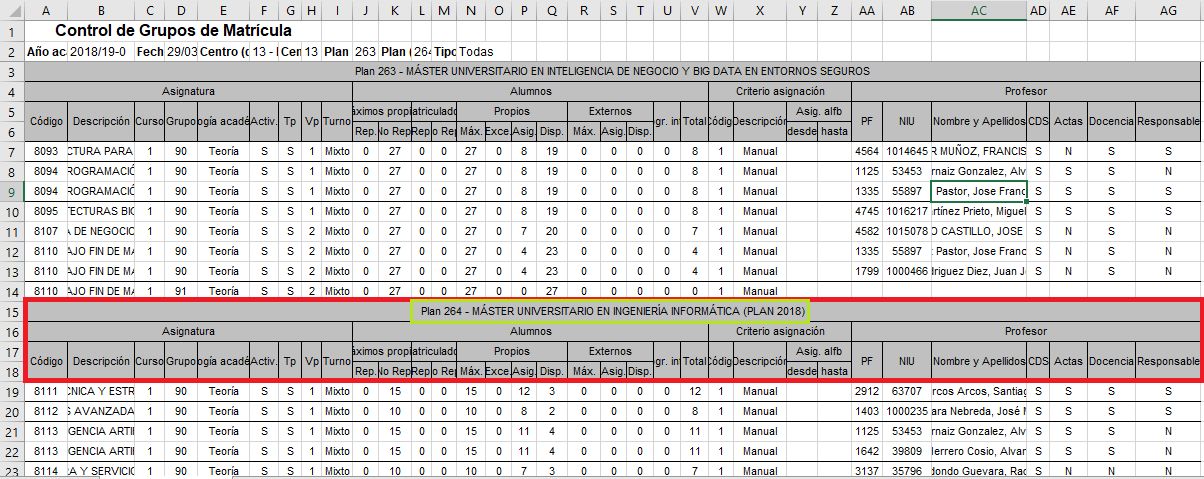
\includegraphics[angle=90, scale = 0.60]{datosFicheroOriginalRojo}
%\imagen{datosFicheroOriginalRojo}{Datos del fichero original}

De esta manera, obtenemos:
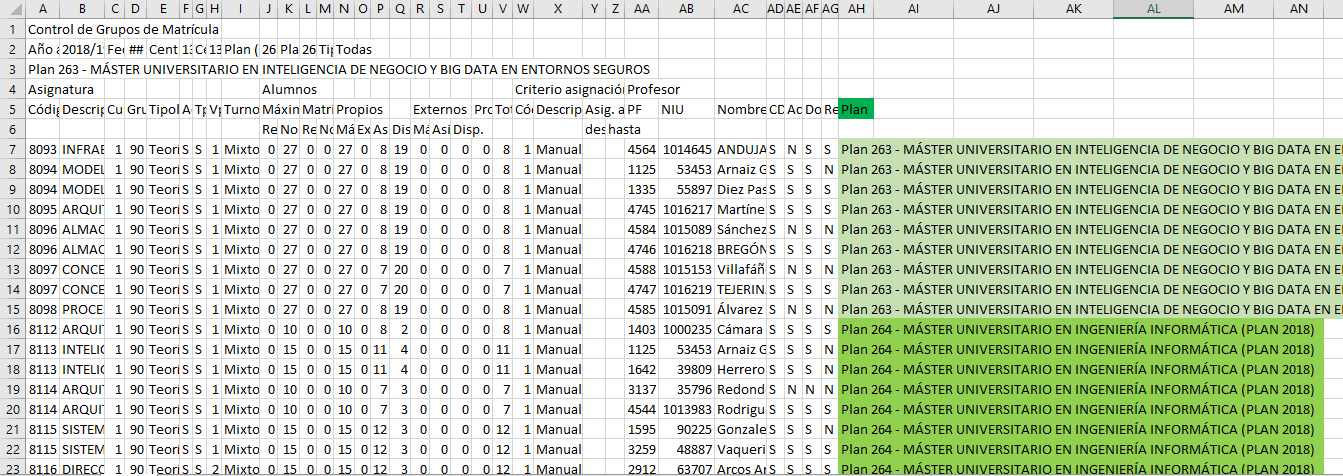
\includegraphics[angle=90, scale = 0.60]{datosFicheroCSVColumnaAnadida}
%\imagen{datosFicheroCSVColumnaAnadida}{Datos del fichero parseado con columna añadida}







  


%\capitulo{6}{Trabajos relacionados}

Para comenzar este apartado, hay que exponer que existen o podrían existir tantos sistemas de información, como empresas u organizaciones encontramos alrededor del mundo. 
Esto es así ya que cada empresa u organización posee una estructura y características muy diferenciadas que la hacen única.

Por lo tanto, hay que destacar que existen numerosos trabajos y libros sobre sistemas de información, que explican conceptos teóricos, así como la forma de implantar estos sistemas.  

Se ha encontrado numerosa documentación sobre sistemas de información geográfica y para el ámbito administrativo. Un libro de carácter teórico, donde se explican características, categorías y el funcionamiento de los diferentes tipos de sistemas sería el siguiente \emph{Introducción a la gestión de sistemas de información en la empresa}\cite{trabajos}.


También existe bastante documentación y trabajos sobre principios de los sistemas de información donde se explica el uso, desarrollo e implantación de los sistemas de información orientados al negocio\cite{effy}.

Como conclusión de este apartado, destacar que no se han encontrado trabajos de investigación muy similares al proyecto realizado, si bien es cierto que como se ha comentado, existen numerosos desarrollos de otros tipos de sistemas u orientados a otro tipo de soluciones.
%\capitulo{7}{Conclusiones y Líneas de trabajo futuras}

Todo proyecto debe incluir las conclusiones que se derivan de su desarrollo. Éstas pueden ser de diferente índole, dependiendo de la tipología del proyecto, pero normalmente van a estar presentes un conjunto de conclusiones relacionadas con los resultados del proyecto y un conjunto de conclusiones técnicas. 
Además, resulta muy útil realizar un informe crítico indicando cómo se puede mejorar el proyecto, o cómo se puede continuar trabajando en la línea del proyecto realizado. 



\bibliographystyle{plain}
\bibliography{bibliografia}

\end{document}
